\documentclass[tikz, margin=3.14mm]{standalone}
\usetikzlibrary{backgrounds}

\begin{document}
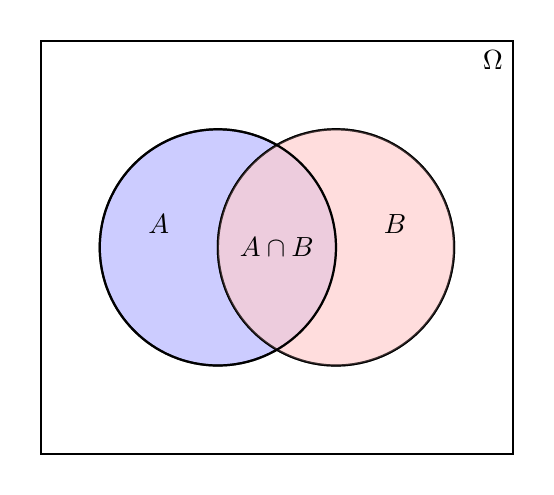
\begin{tikzpicture}[scale=1.5, background rectangle/.style={fill=white}, show background rectangle]
    % Draw the universe rectangle
    \draw[thick] (-2,-1.75) rectangle (2,1.75) node[below left] {\(\Omega\)};
  
    % Draw the fill for circle A and label it
    \draw[thick, fill=blue!20, draw opacity = .65] (-0.5,0) circle (1);
    \node at (-1, 0.2) {\(A\)};
  
    % Draw circle B and label it
    \draw[thick] (0.5,0) circle (1);
    \draw[thick, fill=red!20, opacity = .65] (0.5,0) circle (1);

    % Draw the outer circle for A so it appears "on top of" the intersection
    \node at (1,0.2) {\(B\)};

    %
    \draw[thick] (-0.5,0) circle (1);
  
    % Label the intersection (A \cap B)
    \node at (0,0) {\(A \cap B\)};
  \end{tikzpicture}
\end{document}